\subsection{Ca sử dụng tạo chuyến đi mặc định}
\vspace{0.5cm}


\noindent 
\begin{tabularx}{\linewidth}{| l | X |} 
\hline 
\textbf{Mô tả} & Người dùng có thể tạo chuyến đi để lên kế hoạch du lịch cho bản thân và bạn bè. \\ 
\hline 
\textbf{Luồng cơ bản} & 1. Người dùng bấm vào tab chuyến đi. \newline
                        2. Người dùng bấm vào dấu "+" góc phải trên. \newline
                        3. Hệ thống hiển thị hộp thoại yêu cầu người dùng nhập tên cho chuyến đi. \newline
                        4. Người dùng nhập tên chuyến đi. \newline
                        5. Người dùng bấm "Tạo". \newline
                        6. Hệ thống tạo một chuyến đi mới với tên đã đặt. \\
                        
\hline 
\textbf{Luồng thay thế} & Hệ thống thông báo lỗi khi tên chuyến đi dài hơn 80 kí tự. \\

                       
\hline 
\textbf{Tiền điều kiện} &- Người dùng đang đăng nhập và phiên đăng nhập chưa kết thúc.
                         \\
\hline 
\textbf{Hậu điều kiện} & - Hệ thống thêm chuyến đi với trạng thái là riêng tư của người dùng vào cơ sở dữ liệu.\\

                       

\hline 
\textbf{Yêu cầu phi chức năng} & Hệ thống tạo chuyến đi dưới 2s \\ 
\hline 
\end{tabularx}



\noindent 
\begin{tabular}{| c | c |}
    \hline
    \textbf{Biểu đồ hoạt động} & \textbf{Quan hệ} \\ 
    \hline
    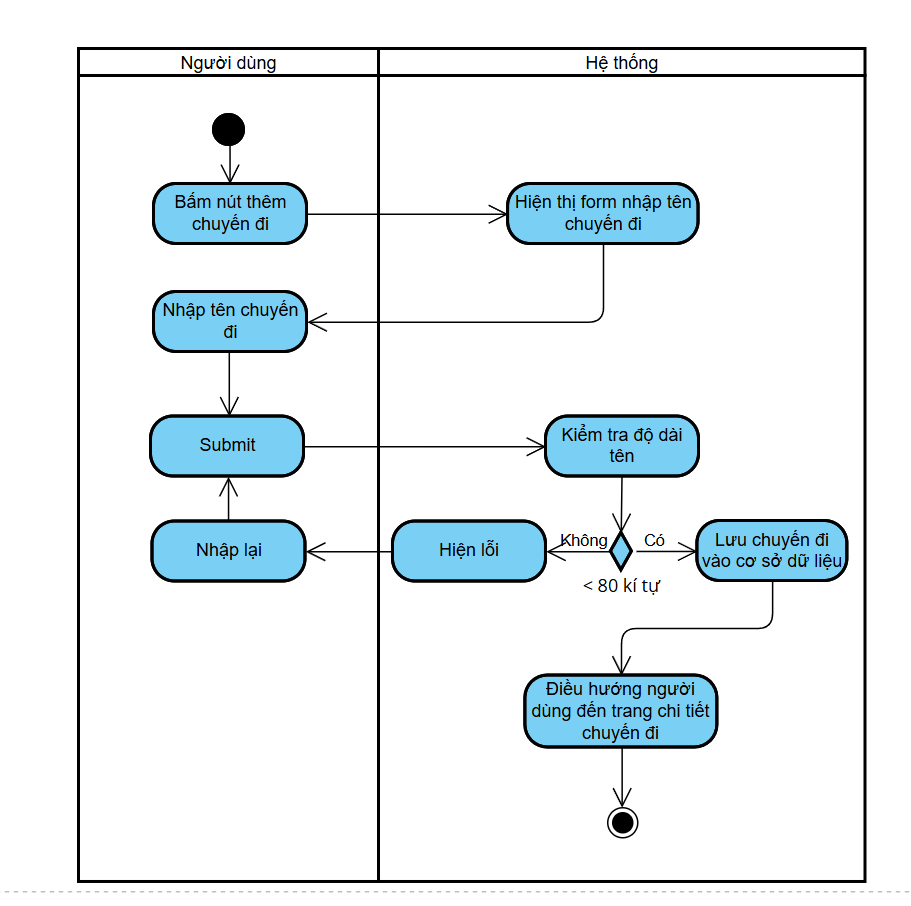
\includegraphics[width=0.5\linewidth]{figures/c3/3-3-11-ad.png} 
    & 
    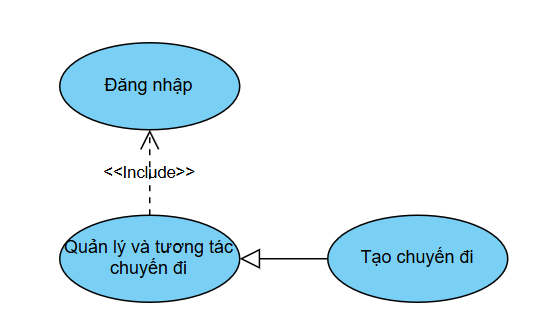
\includegraphics[width=0.45\linewidth]{figures/c3/3-3-11-rd.png} \\ 
    \hline
\end{tabular}


\vspace{0.8cm}

\begin{figure}[H]
    \centering  
    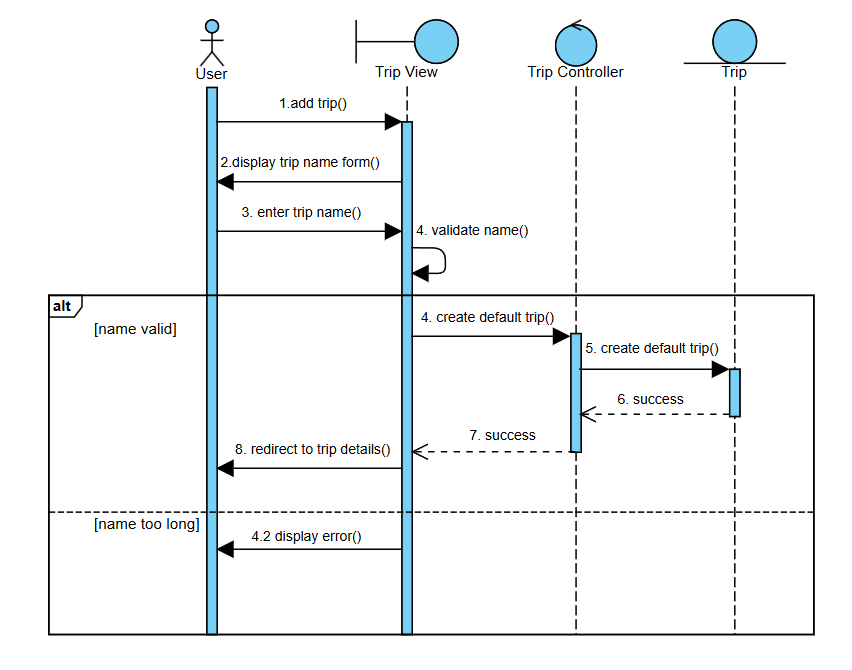
\includegraphics[width=1\textwidth]{figures/c3/3-3-11-sd.png}
    \caption{Biểu đồ tuần tự ca sử dụng tạo chuyến đi mặc định.}
    \label{fig:3-3-11-sequence-diagram}
\end{figure}